\documentclass{standalone}

\usepackage{bm}
\usepackage{fontspec}
\usepackage{tikz}

\usetikzlibrary{arrows.meta}
\usetikzlibrary{backgrounds}
\usetikzlibrary{fit}
\usetikzlibrary{matrix}
\usetikzlibrary{positioning}
\usetikzlibrary{shapes.geometric}

\newcommand{\mat}[1]{\bm{#1}}
\newcommand{\Tr}{^{\top}}
\newcommand{\vc}[1]{\bm{#1}}

\setmainfont{Liberation Sans}
\newlength{\mywidth}
\newlength{\myheight}

\begin{document}
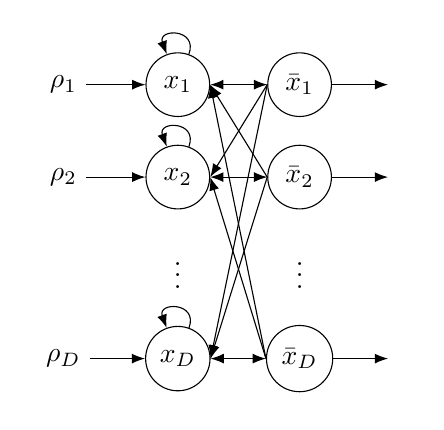
\begin{tikzpicture}[
    every path/.style={-{Latex}},
    inhibit/.style={-{Circle}},
    neuron/.style={circle, minimum size=23, draw=black},
    gate/.style={diamond, draw=black},
    net/.style={rectangle, draw=black},
    ]

    \matrix [column sep=20, row sep=10] {
        \node (rho1) {$\rho_1$}; & \node (x1) [neuron] {$x_1$}; & \node (bar-x1) 
        [neuron] {$\bar{x}_1$}; & \node (out1) {}; \\
        \node (rho2) {$\rho_2$}; & \node (x2) [neuron] {$x_2$}; & \node (bar-x2) 
        [neuron] [neuron] {$\bar{x}_2$}; & \node (out2) {}; \\
        & \node {$\vdots$}; & \node {$\vdots$}; & \\
        \node (rhoD) {$\rho_D$}; & \node (xD) [neuron] {$x_D$}; & \node (bar-xD) 
        [neuron] {$\bar{x}_D$}; & \node (outD) {}; \\
    };

    \foreach \i in {1, 2, D} {
        \draw [loop above, min distance=10, in=110, out=70] (x\i) to (x\i);
        \draw (rho\i) to (x\i);
        \draw (x\i) [{Latex}-{Latex}] to  (bar-x\i);
        \draw (bar-x\i) to (out\i);
    }
    \foreach \i/\j in {1/2, 1/D, 2/1, 2/D, D/1, D/2} {
        \draw (bar-x\i.west) to (x\j.east);
    }


    %\begin{scope}[every path/.style={inhibit}, every to/.style={bend left, 
            %out=45, in=135}]
        %\draw (cs1) to (cs2);
        %\draw (cs2) to (cs1);
        %\draw (cs2) to (cs3);
        %\draw (cs3) to (cs2);
        %\draw (cs1) to (cs3);
        %\draw (cs3) to (cs1);
    %\end{scope}
    %\begin{scope}[every to/.style={loop left, min distance=8, out=200, in=160}]
        %\draw (cs1) to (cs1);
        %\draw (cs2) to (cs2);
        %\draw (cs3) to (cs3);
    %\end{scope}

    %\begin{scope}[every path/.style={inhibit}]
        %\draw (cs1) -> (inv1);
        %\draw (inv1) -> (g1);
        %\draw (cs2) -> (inv2);
        %\draw (inv2) -> (g2);
        %\draw (cs3) -> (inv3);
        %\draw (inv3) -> (g3);
    %\end{scope}

    %\begin{scope}[every path/.style={-}]
        %\draw (c1) -- (g3);
        %\draw (c2) -- (g2);
        %\draw (c3) -- (g1);
    %\end{scope}

    %\node (cue-wta) [rectangle, draw=black, inner sep=10, xshift=-2.5, fit=(cs1) 
    %(cs2) (cs3)] {};
    %\node (cue-wta-lbl) [left=0 of cue-wta] {WTA};
    %\node (n) [below=.7 of cue-wta] {noise};
    %\draw (n) -> (cs1);
    %\draw (n) -> (cs2);
    %\draw (n) -> (cs3);
    %\node (t) [net, right=of cue-wta] {reset signal};
    %\draw [inhibit] (t) -> (cue-wta);

    %\node (pc) [net, right=2 of g2] {primary cue};
    %%\node (cc) [net, above=of pc] {combined cues};
    %%\draw (pc) -> (cc);
    %\node (pcc) [left=0.3of pc] {};
    %\begin{scope}[every path/.style={-}]
        %\draw (g1) -| (pcc.center);
        %\draw (g2) -- (pcc.center);
        %\draw (g3) -| (pcc.center);
    %\end{scope}
    %\draw (pcc.center) -> (pc);

    %%\draw (c1) ++(13mm, 0) |- ([yshift=1.5mm]cc.west);
    %%\draw (c2) ++(11.5mm, 0) |- (cc);
    %%\draw (c3) ++(10mm, 0) |- ([yshift=-1.5mm]cc.west);

    %\node (wta) [net, above right=0.5 and 2 of pc, anchor=north west, minimum 
    %size=60] {WTA};
    %\node (ri) [net, right=of wta] {response inhibition};
    %\draw (wta) to [bend left] (ri);
    %\draw [inhibit] (ri) to [bend left] (wta);
    %\draw ([xshift=10]wta.north) to [bend right, min distance=20, in=280, 
    %out=260] node (wta-north) [] {} ([xshift=-10]wta.north);
    %\draw ([xshift=10]ri.north) to [bend right, min distance=20, in=280, 
    %out=260] ([xshift=-10]ri.north);
    %\draw (pc) -- node [pos=0.3, above] {$\tilde{\mat A}$} (pc-|wta.west);
    %\node (r) [below=1.5 of wta, net] {response};
    %\draw (wta) -> (r);

    %\begin{scope}[on background layer, rounded corners, inner sep=5]
        %\node (cue-sel) [fit=(cue-wta) (cue-wta-lbl) (n) (pc) (g1) (g2) (g3) 
        %(t), fill=red!20] {};
        %\node (res-net) [fit=(wta) (wta-north.center) (ri), fill=blue!20] {};

        %\draw ([yshift=3]bias.east) -> ([yshift=3]inv1.west);
        %\draw (bias) -> (inv2);
        %\draw ([yshift=-3]bias.east) -> ([yshift=-3]inv3.west);
    %\end{scope}
    %\node [above=0 of cue-sel] {cue selection};
    %\node [above=0 of res-net] {response network};

    %\node [matrix, column 2/.style={anchor=west}, row sep=3] at (12.5, -2.5) {
        %\node [neuron] {}; & \node {Group of neurons}; \\
        %\node [net] {net}; & \node {Network of neurons}; \\
        %\node [gate] {}; & \node {Gating neurons}; \\
        %\draw (-0.3, 0) -> (.3, 0); & \node {Flow of information}; \\
        %\draw [inhibit] (-0.3, 0) -> (.3, 0); & \node {Inhibitory connection}; 
        %\\
    %};
\end{tikzpicture}
\end{document}
